\renewcommand{\theparagraph}{A}

\section{SINR derivation}\label{appA:SINR_deriv}
Let $A$ and $B$ be 2 \gls{rv}'s. These basics properties will be used:
\begin{equation}
    \begin{split}
        &\EX{\alpha A + \beta B} = \alpha \EX{A} + \beta \EX{B} \; \;\; \;\alpha,\beta\in\R \\
        &\EX{AB} = \EX{A} \EX{B} \; \;\; \; \text{if $A$ and $B$ are independent} \\
        &\EX{AB} = \EX{A} \EX{B} + \text{cov}(A,B)\; \; \; \;\text{if $A$ and $B$ are correlated}
    \end{split} 
\end{equation}
\subsection{At the intended position}
As a recall, the received sequence is given by:
\begin{equation}
    \textbf{y}_{\text{B}}^H = \sqrt{\alpha} \; \spread^H \module{\HB}^2 \spread \textbf{x} \;  +  \;  \spread^H \textbf{v}_\text{B} 
    \label{eq:app:rx_bob_AN}
\end{equation}
From (\ref{eq:RV_sinr_b}) and (\ref{eq:expected_bob}), we have:

\begin{subequations}
    \begin{align}
        \EX{|k|^2} &= \EX{\module{\sqrt{\alpha}\spread^H \module{\HB^2} \spread}^2} \\
        \EX{|k_n|^2} &=\EX{\left|\frac{\sqrt{\alpha}}{U}\sum_{i=0}^{U-1} \left| h_{\text{B}, n + iN}\right|^2\right|^2}  \\
        &= \frac{\alpha}{U^2} \EX{\left(\sum_{i=0}^{U-1} \left| h_{\text{B}, n + iN}\right|^2\right) \left(\sum_{j=0}^{U-1} \left| h_{\text{B}, n + jN}\right|^2\right)^H} \label{subeq:appA:comp1}\\
        &= \frac{\alpha}{U^2}\EX{\sum_{i=0}^{U-1}\sum_{j=0}^{U-1}\left| h_{\text{B}, n + iN}\right|^2 | h^*_{\text{B}, n + jN}|^2} \\
        &= \frac{\alpha}{U^2}\EX{\sum_{i=0}^{U-1}\left| h_{\text{B}, n + iN}\right|^4 + \sum_{i=0}^{U-1}\sum_{\substack{j=0 \\ j\neq i}}^{U-1}\left| h_{\text{B}, n + iN}\right|^2 | h^*_{\text{B}, n + jN}|^2} \\
        &= \frac{\alpha}{U^2} \left(\EX{\sum_{i=0}^{U-1}\left| h_{\text{B}, n + iN}\right|^4} + \EX{\sum_{i=0}^{U-1}\sum_{\substack{j=0 \\ j\neq i}}^{U-1}\left| h_{\text{B}, n + iN}\right|^2 | h^*_{\text{B}, n + jN}|^2} \right) \\
        &=  \frac{\alpha}{U^2} \left(\EX{\sum_{i=0}^{U-1}\left| h_{\text{B}, n + iN}\right|^4} + \EX{\sum_{i=0}^{U-1}\left| h_{\text{B}, n + iN}\right|^2}\EX{\sum_{\substack{j=0 \\ j\neq i}}^{U-1} | h^*_{\text{B}, n + jN}|^2} \right) \label{eq:an_2g}\\
        &= \frac{\alpha}{U^2} \left( 2U + U(U-1)\right) = \frac{\alpha (U+1)}{U} \label{eq:an_2h}
    \end{align}
    \label{eq:appA:data_bob}
\end{subequations}
Going from (\ref{eq:an_2g}) to (\ref{eq:an_2h}) arises from the fact that $\EX{x f(x)} = \EX{\frac{\partial f(x)}{\partial x^*}}$. It is then easy to show that $\EX{\left| h_{\text{B}, n + iN}\right|^4}=2$. \\
For the data symbol we have by definition $\EX{|x_n|^2}=1$, and for the noise symbol, we obtain:
\begin{subequations}
    \begin{align}
        \EX{|\textbf{v}_{\text{B}}|^2} &=  \EX{\module{\spread^H \vb}^2} \\
        &= \EX{\left(\spread^H \vb \right)\left(\spread^H \vb \right)^H} \\
        &=\EX{\spread^H \vb \vb^* \spread } \\
        \EX{|v_{\text{B,n}}|^2} &= \frac{1}{U} \EX{\sum_{i=0}^{U-1} |v_{\text{B}, n + iN}|^2} = \sigma^2_{\text{V,B}}
    \end{align}
    \label{eq:appA:noise_bob}
\end{subequations}

       % &\EX{|x_n|^2} = 1\\
       % &\EX{|v_{B,n}|^2} = \sigma^2_{V,E}



\subsection{At the unintended position}
At the unintended position, the received signal is given by:
\begin{equation}
    \textbf{y}_{\text{E}}^G = \sqrt{\alpha} \textbf{G}\Gamma_{\text{E}} \textbf{x} + \sqrt{1-\alpha} \textbf{G} \HE \w + \ve
    \label{eq:appA_rx_eve}
\end{equation}
where $\Gamma_{\text{E}} = \HE \HB^*\spread$




\subsubsection{Eve and Bob with identical capacities}
In this scenario, we have:
\begin{equation}
    \textbf{y}_{\text{E}}^G = \sqrt{\alpha} \spread^H \Gamma_{\text{E}} \spread\; \textbf{x} \; +  \; \sqrt{1-\alpha} \; \spread^H \HE \w  \; +  \; \spread^H  \textbf{v}_\text{E} 
    \label{eq:app:rx_eve_filt0}
\end{equation}
From (\ref{eq:expected_eve_filt0}), we have:
\begin{subequations}
    \begin{align}
        \EX{|\textbf{A}_{1}|^2} &= \EX{\module{\sqrt{\alpha}\spread^H \HE\HB^* \spread}^2} \\
        &= \alpha \EX{\left( \spread^H \HE\HB^* \spread \right) \left( \spread^H \HE\HB^* \spread\right)^H} \\
        \EX{|A_{1,n}|^2}&=\alpha \EX{\frac{1}{U^2} \sum_{i=0}^{U-1} \left| h_{\text{E}, n + iN} \right|^2 \left| h^*_{\text{B}, n + iN}\right|^2 } \\
        &= \frac{\alpha}{U}
    \end{align}
    \label{eq:appA:data_eve_filt0}
\end{subequations}
For the noise component:
\begin{subequations}
    \begin{align}
        \EX{|\textbf{A}_{2}|^2} &=  \EX{\module{\spread^H \ve}^2} \\
        &= \EX{\left(\spread^H \ve \right)\left(\spread^H \ve \right)^H} \\
        &=\EX{\spread^H \ve \ve^* \spread } \\
        \EX{|A_{2,n}|^2} &= \frac{1}{U} \EX{\sum_{i=0}^{U-1} |v_{\text{E}, n + iN}|^2} = \sigma^2_{\text{V,E}}
    \end{align}
    \label{eq:appA:noise_eve_filt0}
\end{subequations}
The \gls{an} term is given by:
\begin{subequations}
    \begin{align}
        \EX{|\textbf{A}_{3}|^2} &=  \EX{\module{\sqrt{1-\alpha}\spread^H \HE \w}^2} \\
        &= (1-\alpha)\EX{\left(\spread^H \HE \w \right)\left(\spread^H \HE\w \right)^H} \\
        &=(1-\alpha)\EX{\spread^H \HE\textbf{H}^*_{\text{E}} \w\w^* \spread } \\
        \EX{|A_{3,n}|^2}  &= \frac{1-\alpha}{U} \EX{\sum_{i=0}^{U-1} |h_{\text{E}, n + iN}w_{n + iN}|^2} = (1-\alpha)\sigma^2_{\text{AN}}
    \end{align}
    \label{eq:appA:an_eve_filt0}
\end{subequations}



\subsubsection{Matched Filtering}
When Eve performs a matched filtering with the received signal, we obtain:
\begin{equation}
    \textbf{y}_{\text{E}}^G = \sqrt{\alpha} \spread^H \module{\HE}^2 \module{\HB}^2 \spread\; \textbf{x} \; +  \; \sqrt{1-\alpha} \; \spread^H \HB\module{\HE}^2 \w  \; +  \; \spread^H  \textbf{H}^*_E \textbf{H}_B \;\ve
    \label{eq:appA:rx_eve_filt1}
\end{equation}
The data component is given by:
\begin{subequations}
    \begin{align}
        \EX{|\textbf{A}_{1}|^2} &= \EX{\module{\sqrt{\alpha} \spread^H \module{\HE}^2 \module{\HB}^2 \spread\; \textbf{x}}^2} \\
        &= \alpha \EX{\module{ \spread^H \module{\HE}^2 \module{\HB}^2 \spread}^2} \EX{|\textbf{x}|^2} \\
        \EX{|A_{1,n}|^2} &= \alpha \EX{\left|\frac{1}{U}\sum_{i=0}^{U-1} \left| h_{\text{B}, n + iN}\right|^2 \left| h_{\text{E}, n + iN}\right|^2\right|^2} \\
        &=  \frac{\alpha}{U^2} \EX{\left(\sum_{i=0}^{U-1} \left| h_{\text{B}, n + iN}\right|^2 \left| h_{\text{E}, n + iN}\right|^2 \right) \left(\sum_{j=0}^{U-1} \left| h_{\text{B}, n + jN}\right|^2 \left| h_{\text{E}, n + iN}\right|^2 \right)^H} \label{subeq:appA_comp2} \\
        &= \frac{\alpha}{U^2} \EX{\sum_{i=0}^{U-1}\sum_{j=0}^{U-1} \left| h_{\text{B}, n + jN}\right|^2 \left| h_{\text{E}, n + iN}\right|^2 \left| h^*_{\text{B}, n + jN}\right|^2 \left| h^*_{\text{E}, n + iN}\right|^2} \\
        &= \frac{\alpha}{U^2}\left( \sum_{i=0}^{U-1} \left| h_{\text{B}, n + jN}\right|^4 \left| h_{\text{E}, n + iN}\right|^4 + \sum_{i=0}^{U-1}\sum_{\substack{j=0 \\ j\neq i}}^{U-1}  \left| h_{\text{B}, n + jN}\right|^2 \left| h_{\text{E}, n + iN}\right|^2 \left| h^*_{\text{B}, n + jN}\right|^2 \left| h^*_{\text{E}, n + iN}\right|^2 \right) \\
        &= \frac{\alpha}{U^2} \left(U.2.2 + U(U-1) \right) = \frac{\alpha (U+3)}{U}
        \label{subeq:appA_match_final}
    \end{align} 
    \label{eq:appA:data_eve_filt1}
\end{subequations}
We remark that (\ref{subeq:appA_comp2}) can be directly computed from (\ref{subeq:appA:comp1}), which leads to (\ref{subeq:appA_match_final}).\\

The noise component is:
\begin{subequations}
    \begin{align}
        \EX{|\textbf{A}_{2}|^2} &=  \EX{\module{\spread^H \HE^* \HB \ve}^2} \\
        &= \EX{\left(\spread^H \HE^* \HB \ve \right)\left(\spread^H \HE^* \HB \ve \right)^H} \\
        &=\EX{\spread^H   \HE \HE^* \HB\HB^*  \ve \ve^* \spread } \\
       \EX{|A_{2,n}|^2} &= \frac{1}{U} \EX{\sum_{i=0}^{U-1} |h_{\text{E}, n + iN}|^2 |h_{\text{B}, n + iN}|^2 |v_{\text{E}, n + iN}|^2} = \sigma^2_{\text{V,E}}
    \end{align}
    \label{eq:appA:noise_eve_filt1}
\end{subequations}
The \gls{an} component is:
\begin{subequations}
    \begin{align}
        \EX{|\textbf{A}_{3}|^2} &= \EX{\module{\sqrt{1-\alpha} \; \spread^H \HB\module{\HE}^2 \w}^2} \\
        &= (1-\alpha) \EX{\left(\spread^H \HB\module{\HE}^2 \w \right)\left(\spread^H \HB\module{\HE}^2 \w\right)^H} \\
        \EX{|A_{3,n}|^2} &= \frac{1-\alpha}{U} \EX{\sum_{i=0}^{U-1}  |h_{\text{B}, n + iN}|^2 |h_{\text{E}, n + iN}|^4 |w_{n + iN}|^2} \label{eq:appA_an_filt1_c} \\ 
        &= 2(1-\alpha) \left( \sigma^2_{\text{AN}} + \text{cov}(\module{\w}^2,\module{\textbf{H}_\text{B}}^2) \right) \label{eq:appA_an_filt1_d}
    \end{align}
\end{subequations}
Since the \gls{an} signal and Bob channel are not independent, we cannot compute the expectations in (\ref{eq:appA_an_filt1_c}) separately. This is why we have  to add the covariance in (\ref{eq:appA_an_filt1_d}).
 %   \EX{|A_{3,n}|^2} = 2(1-\alpha) \left( \sigma^2_{\text{AN}} + \text{cov}(\module{\w}^2,\module{\textbf{H}_\text{B}}^2) \right)
%\end{equation}








\subsubsection{AN suppression}
In this scenario, the received signal at Eve is given by:
\begin{equation}
    \textbf{y}_{\text{E}}^G = \sqrt{\alpha} \spread^H \module{\HB}^2 \spread\; \textbf{x} \; +  \; \spread^H  \HE^{-1} \textbf{H}_B \;\ve
    \label{eq:appA:rx_eve_filt2}
\end{equation}
In what concerns the data component, the computation is straightforward since it is similar to (\ref{eq:appA:data_bob}). We then obtain $ \EX{|A_{1,n}|^2} = \alpha \frac{U+1}{U}$.\\
The noise term is:
\begin{subequations}
    \begin{align}
        \EX{|\textbf{A}_{2}|^2} &=  \EX{\module{\spread^H \HB \HE^{-1} \ve}^2} \\
        &= \EX{\left(\spread^H \HB \HE^{-1} \ve \right)\left(\spread^H \HB \HE^{-1} \ve \right)^H} \\
        &=\EX{\spread^H   \module{\HB}^2 \module{\HE^{-1}}^2 \module{\ve}^2 \spread } \\
        \EX{|A_{2,n}|^2} &= \frac{1}{U} \EX{\sum_{i=0}^{U-1} |h_{\text{E}, n + iN}^{-1}|^2 |h_{\text{B}, n + iN}|^2 |v_{\text{E}, n + iN}|^2} \\
        &= \sigma^2_{\text{V,E}}\;\EX{|h_{\text{E}, n + iN}^{-1}|^2} =  \sigma^2_{\text{V,E}} \;\EX{ \frac{1}{|h_{\text{E}, n + iN}|^2}} \label{eq:appA:noise_filt2_e}
    \end{align}
    \label{eq:appA:noise_eve_filt2}
\end{subequations}
The issue that arises in (\ref{eq:appA:noise_filt2_e}) is that the variable $X = \frac{1}{|h_{\text{E}, n + iN}|^2}$ follows an inverse chi-square distribution of $\nu=2$ degrees of freedom. The expected value of such a distribution is given by:
\begin{equation}
    \EX{X} = \frac{1}{\nu - 2} = + \infty
    \label{eq:appA_mean_noise_filt2}
\end{equation}
Eq. (\ref{eq:appA_mean_noise_filt2}) suggests that the expected value of the energy of the noise component is infinite which implies that the ergodic \gls{sinr} at Eve tends to zero and that the ergodic \gls{sr} of the communication tends to the ergodic capacity of Bob. However, this is only the case when $|h_{\text{E}, n + iN}|^2 = 0$, i.e. when a subcarrier of Eve's channel has a zero gain. From (\ref{eq:appA:noise_eve_filt2}), we clearly understand that this decoding structure will amplify the noise component which is not optimal, as already anticipated from section \ref{par:perf_an_suppression}. However, we can compute the probability $p$ that our \gls{rv} $X$ is bigger that a certain threshold $t$, i.e., we can compute the upper-bound value of the \gls{sr} with a given probability. The \gls{pdf} of $X$ has the form:
\begin{equation}
    f_X(x) = \frac{2^{-\nu/2}}{\Gamma (\nu/2)} x^{-\nu/2-1} e^{\frac{-1}{2x}}
\end{equation}
where $\Gamma(a) = (a-1)! = \int_0^\infty z^{a-1} e^{-z} dz$ is the Gamma function of the integer $a$. The probability that our \gls{rv} $X$ is bigger than $t$ is given by:
\begin{equation}
    \begin{split}
        Pr( t < X ) &= \int_t^{+\infty} f_X(x) dx = p \\
        \Leftrightarrow & \hspace{.1in} p =  \int_t^{+\infty} \frac{2^{-1}}{\Gamma (1)} x^{-2} e^{\frac{-1}{2x}} dx \\
        \Leftrightarrow & \hspace{.1in} p = \int_{1/t}^0 e^{-u/2} du \\
        \Leftrightarrow & \hspace{.1in} p = 1 - e^{\frac{-1}{2t}}\\
        \Leftrightarrow & \hspace{.1in} t = \frac{-2}{\ln{(1-p)}}
    \end{split}
\end{equation}
This relation is plotted in fig.\ref{fig:cdf_inverse_chi_square} where we see that we have for example a probability of $p=5\%$ that our decoding structure will amplify the noise component by a factor $t=27$.
\begin{figure}[htb!]
    \centering
    \centerline{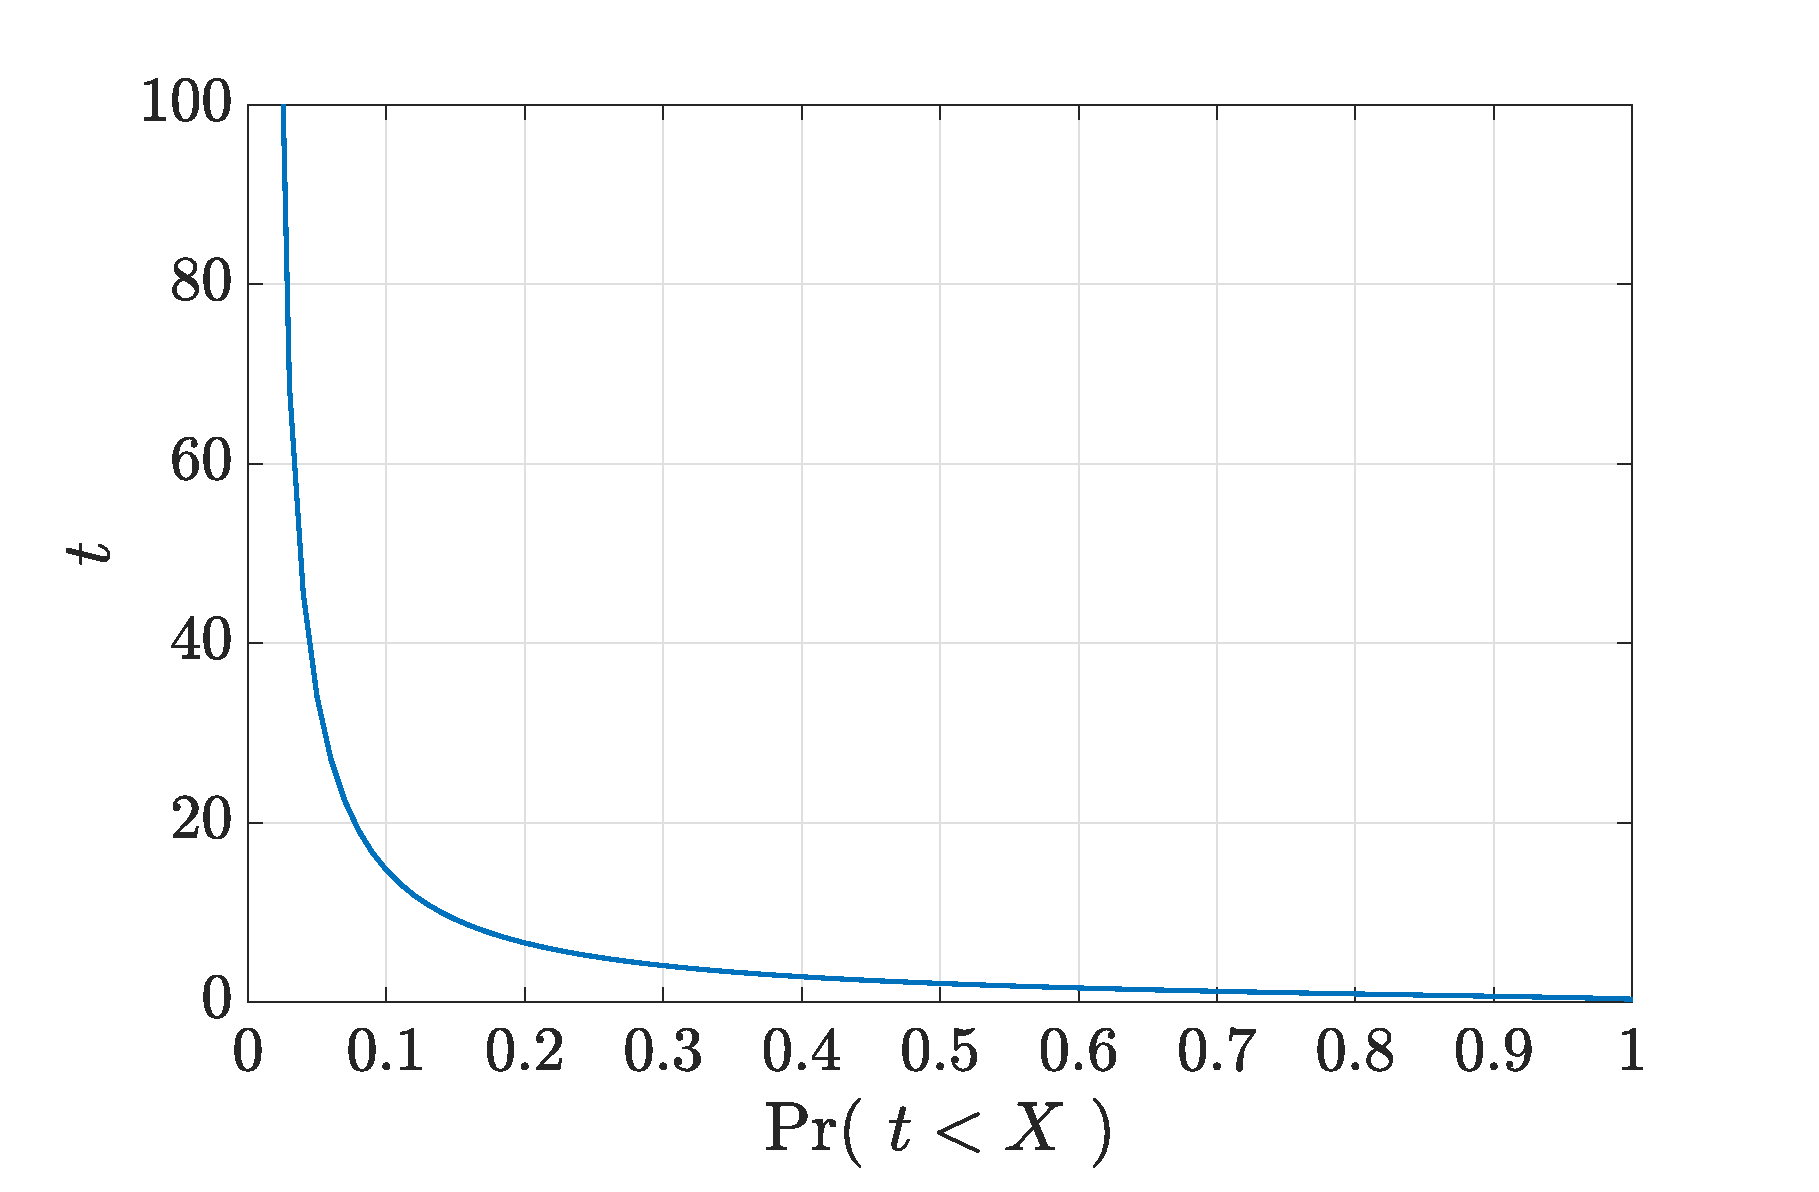
\includegraphics[width = .65\textwidth]{graphs/inverse_chi_square_cdf.eps}}
    \caption{CDF of the inverse chi-square distribution of $\nu = 2$ degrees of freedom.}
    \label{fig:cdf_inverse_chi_square}
\end{figure} 










\subsubsection{LMMSE}
As a recall, the \gls{lmmse} equalizer \textbf{G} needs to satisfy the orthogonality principle. In doing so, we have:
\begin{subequations}
    \begin{align}
         &\EX{(\hat{\textbf{x}}_\text{E} - \textbf{x})\textbf{y}_\text{E}^\text{H}} = \textbf{0} \\
         \Leftrightarrow \; & \EX{(\textbf{G} \textbf{Y}_\text{E}-\textbf{x}) \textbf{y}_\text{E}^\text{H}} = \textbf{0} \\
         \Leftrightarrow \; & \EX{\textbf{G} \textbf{Y}_\text{E} \textbf{y}_\text{E}^\text{H} }  = \EX{\textbf{x} \textbf{y}_\text{E}^\text{H}} \\
         \Leftrightarrow \; & \textbf{G}  = \EX{\textbf{x} \textbf{y}_\text{E}^\text{H}} \left(\EX{\textbf{Y}_\text{E} \textbf{y}_\text{E}^\text{H}}\right)^{-1} \\
         \begin{split}
             \Leftrightarrow \; & \textbf{G}  = \EX{\textbf{x}  \left(   \sqrt{\alpha} \Gamma_{\text{E}} \textbf{x} + \sqrt{1-\alpha} \HE \w + \ve \right)^H }  \\
             & \hspace{.35in} \left(\EX{\left(   \sqrt{\alpha} \Gamma_{\text{E}} \textbf{x} + \sqrt{1-\alpha} \HE \w + \ve \right)\left(   \sqrt{\alpha} \Gamma_{\text{E}} \textbf{x} + \sqrt{1-\alpha} \HE \w + \ve \right)^H}\right)^{-1}
         \end{split}\\
         \begin{split}
            \Leftrightarrow \; & \textbf{G}  = \left(\sqrt{\alpha} \EX{\textbf{xx}^H \Gamma_{\text{E}}^H} + \sqrt{1-\alpha}  \EX{\textbf{x}\w^H \HE^H}  + \EX{x \ve^H}\right) \\
            &\hspace{.35in} \left( \EX{\alpha \Gamma_\text{E} \Gamma_\text{E}^H \textbf{xx}^H + (1-\alpha) \HE \w\w^H\HE^H + \ve\ve^H}\right)^{-1}
         \end{split} \\
         \Leftrightarrow \; & \textbf{G}  = \sqrt{\alpha} \sigma^2_{\text{X}} \Gamma_{\text{E}}^H \left( \alpha \sigma^2_{\text{X}} \Gamma_{\text{E}}\Gamma_{\text{E}}^H  + (1-\alpha) \module{\HE}^2 \sigma^2_{\text{AN}} + \sigma^2_{\text{VE}} \textbf{I}_N\right)^{-1}
    \end{align}
    \label{eq:appA_lmmse}    
\end{subequations}
